\documentclass[a4paper,12pt]{ctexart}
\usepackage{amsmath}
\usepackage{amsfonts}
\usepackage{float}
\usepackage{enumerate}
\usepackage{graphicx}
\usepackage{tikz}
\usepackage{pgfplots}
\usepackage[hidelinks]{hyperref}
\title{经济学综合大作业}
\author{董晨阳 \and 李昭伦 \and 梁予昕}
\date{\today}
\begin{document}
\maketitle
\section{第一题}\label{sec:1}
厂商雇佣资本和劳动,根据边际生产率支付要素价格。
$$\max F(K, L)-(r+\delta)K-wL$$
完全竞争假设,利润为 0。
$$\frac{\partial F(K,L)}{\partial K}=r+\delta$$
故
$$r_t=\alpha Ak_t^{\alpha-1}-\delta$$

劳动的边际产出为
$$\frac{\partial F(K,L)}{\partial L}$$
单位劳动的工资率为
$$W_t=(1-\alpha) Ak_t^\alpha$$
\section{第二题}
对于第一种代理人,由于人口恒定为$\lambda$,人均的预算约束为
\begin{equation*}
    c_{1,t}+\frac{I_{1,t}}{\lambda}=W_tl_{1,t}+R_tk_{1,t}
\end{equation*}
又由于
\begin{equation*}
    K_{1,t+1} = K_{1,t}(1 -\delta) + I_{1,t}
\end{equation*}
可以得到
\begin{equation*}
    g(t)=c_{1,t}+k_{1,t+1} - k_{1,t}(1 -\delta)-W_tl_t-R_tk_{1,t}=0
\end{equation*}
最大化效用有拉格朗日方程
\begin{equation*}
    \mathcal{L}(l_{1,t},c_{1,t},k_{t+1})=\mathbb{E}_t\{\lambda U(l_t,c_t)+\lambda_t g(t)\}
\end{equation*}
F.O.C.
\begin{eqnarray*}
    \frac{\partial \mathcal{L}}{\partial l_{1,t}}&=E_t\{\beta^t(-\frac{b}{1-l_{1,t}}+\lambda_tw_t)\}&=0\\
    \frac{\partial \mathcal{L}}{\partial c_{1,t}}&=E_t\{\beta^t(\frac{1}{c_{1,t}}-\lambda_t)\}&=0\\
    \frac{\partial \mathcal{L}}{\partial k_{t+1}}&=E_t\{-\beta^t\lambda_t+\beta^{t+1}(1+r_{t+1})\lambda_{t+1}\}&=0\\
\end{eqnarray*}
解得消费与闲暇的替代关系为
\begin{equation*}
    \frac{c_{1,t}}{1-l_{1,t}}=\frac{w_t}{b}
\end{equation*}
跨期消费的欧拉方程为
\begin{equation*}
    \frac{1}{c_{1,t}}=\beta E_t\{(1+r_{t+1})\frac{1}{c_{t+1}}\}
\end{equation*}
\section*{第三题}
第二类代理行为人的优化问题为
\begin{equation*}
    \max_{c_{2,t},l_{2,t}} \ln c_{2,t}+b \ln (1-l_{2,t})
\end{equation*}
s.t.
\begin{equation*}
    c_{2,t}=w_tl_{2,t}
\end{equation*}
构造拉格朗日公式F.O.C.
\begin{eqnarray*}
    \frac{1}{c_{2,r}}&=&\lambda_t\\
    \frac{b}{1-l_{2,t}}&=&w_t\lambda_t
\end{eqnarray*}
解得消费与闲暇的替代关系为
\begin{equation*}
    \frac{c_{2,t}}{1-l_{2,t}}=\frac{w_t}{b}
\end{equation*}
该类代理人没有欧拉方程,因为无法跨期配置资源
\section*{第四题}
稳态的结果为:
\begin{table}[H]
    \centering
    \begin{tabular}{l|c}
        y  & 0.559836    \\
        c  & 0.49519     \\
        c1 & 0.373893    \\
        c2 & 0.616488    \\
        i  & 0.129292    \\
        k  & 2.15487     \\
        l  & 0.393512    \\
        l1 & 0.393512    \\
        l2 & 4.29611e-08 \\
        r  & 1.03093     \\
        w  & 0.924732    \\
        a  & 1           \\
    \end{tabular}
\end{table}
\section*{第五题}
200期模拟作图如下:
\begin{figure}[H]
    \begin{minipage}{0.48\linewidth}
        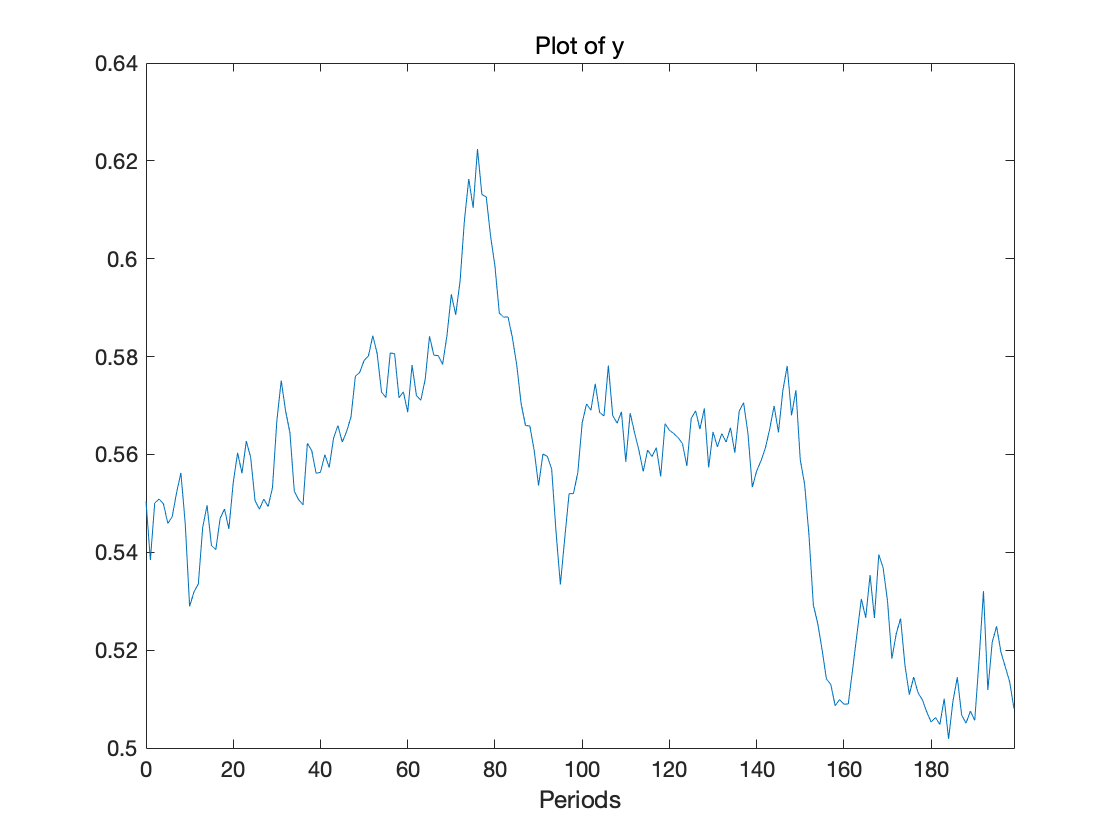
\includegraphics[width=\linewidth]{img/figure3.png}
        \caption{$Y$}
    \end{minipage}
    \begin{minipage}{0.48\linewidth}
        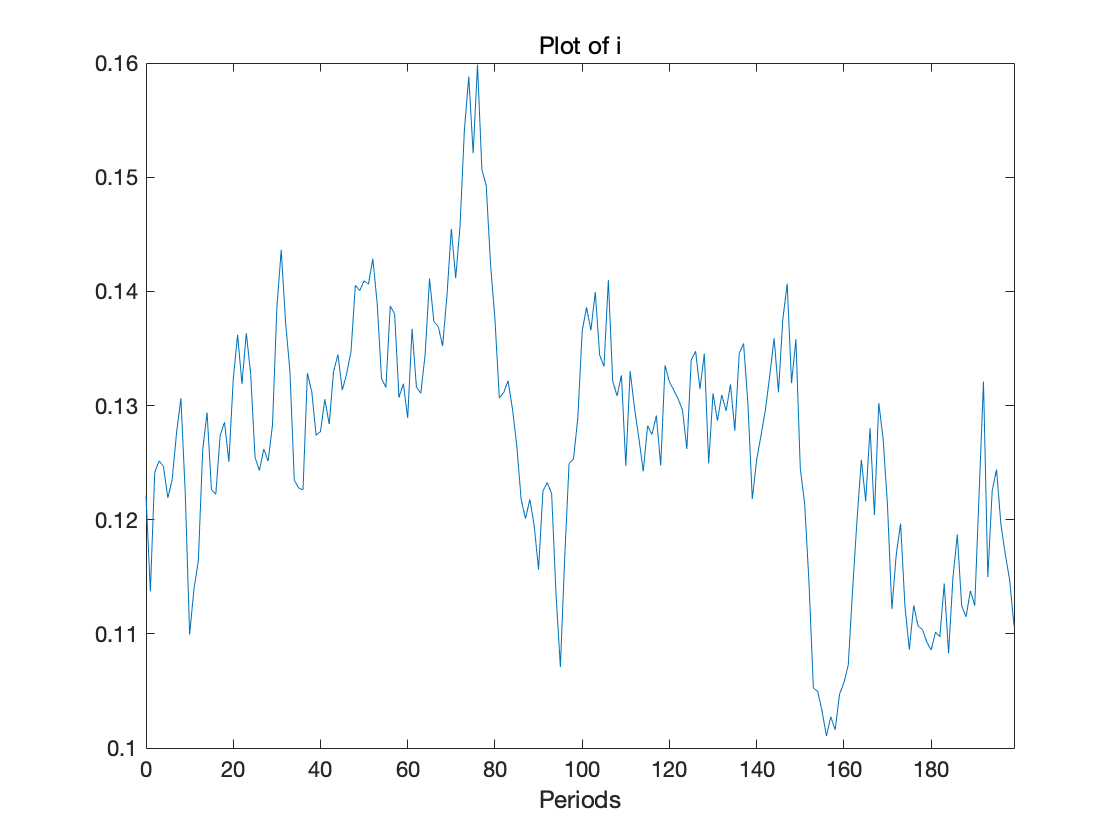
\includegraphics[width=\linewidth]{img/figure4.png}
        \caption{$I$}
    \end{minipage}
\end{figure}
\begin{figure}[H]
    \begin{minipage}{0.48\linewidth}
        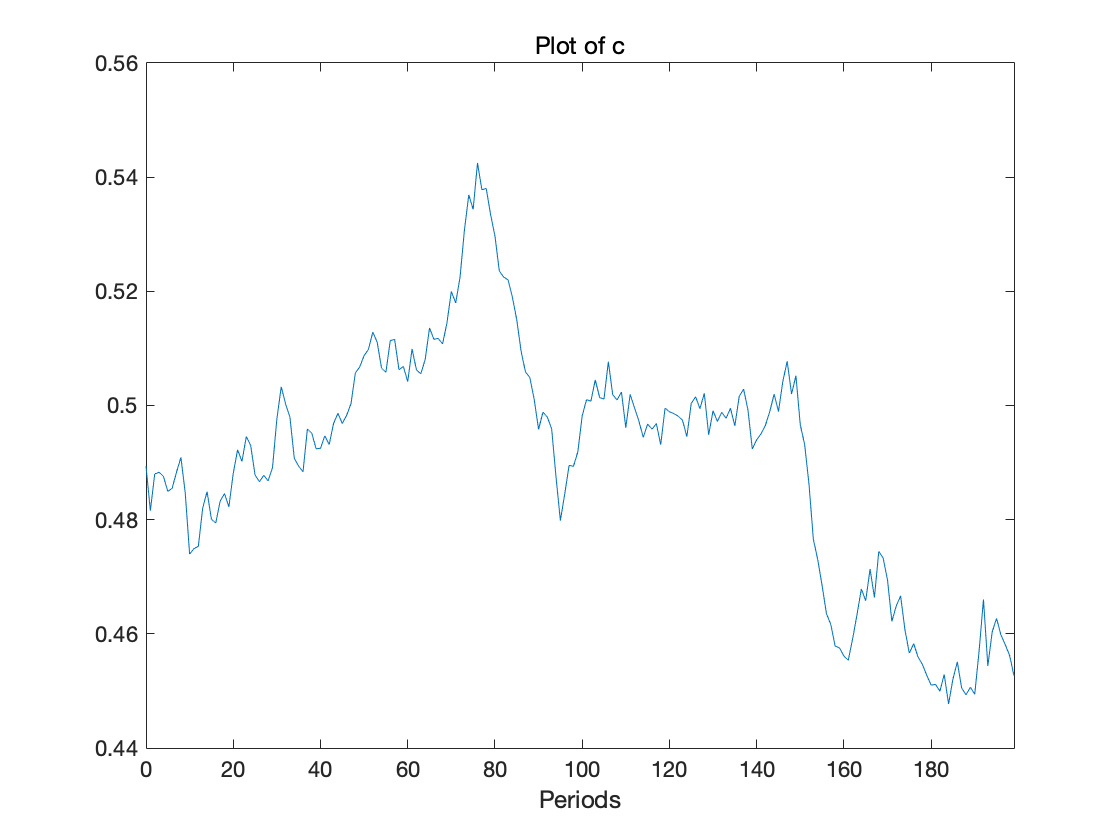
\includegraphics[width=\linewidth]{img/figure5.png}
        \caption{$C$}
    \end{minipage}
    \begin{minipage}{0.48\linewidth}
        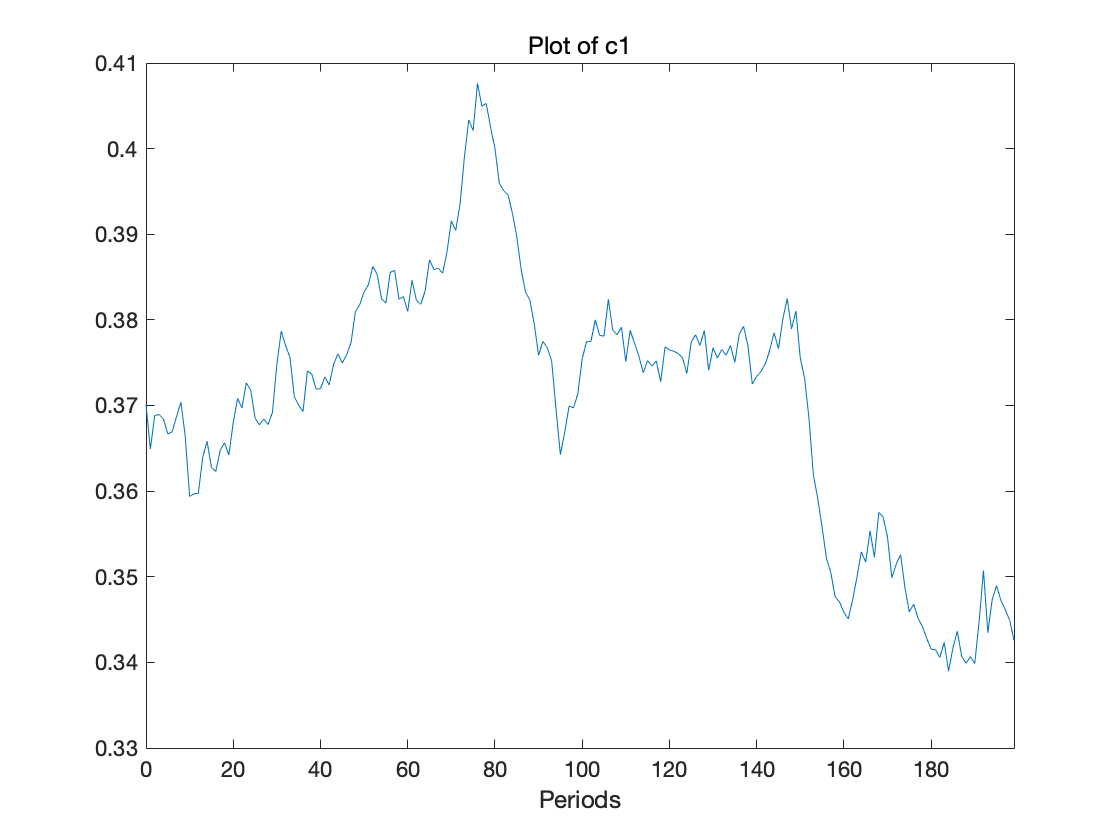
\includegraphics[width=\linewidth]{img/figure6.png}
        \caption{$C_1$}
    \end{minipage}
\end{figure}
\begin{figure}[H]
    \begin{minipage}{0.48\linewidth}
        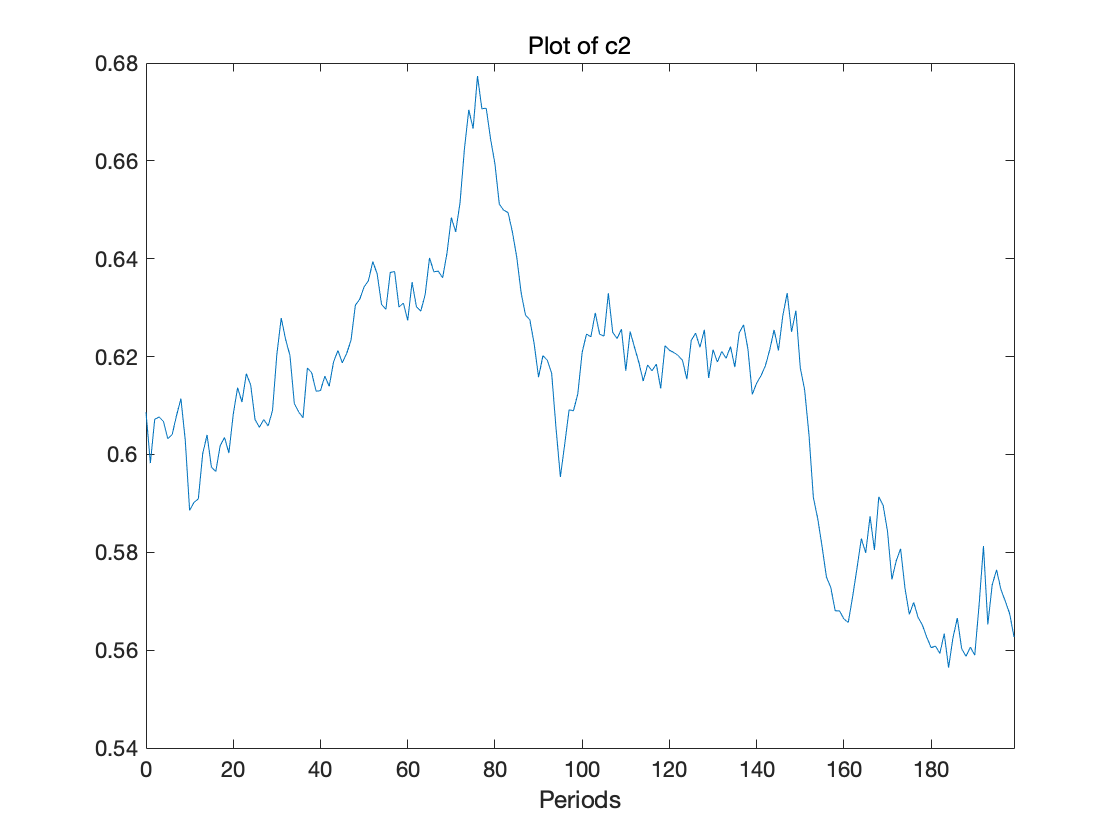
\includegraphics[width=\linewidth]{img/figure7.png}
        \caption{$C_2$}
    \end{minipage}
\end{figure}
\section*{第六题}
两百期模拟脉冲响应函数如下图
\begin{figure}[H]
    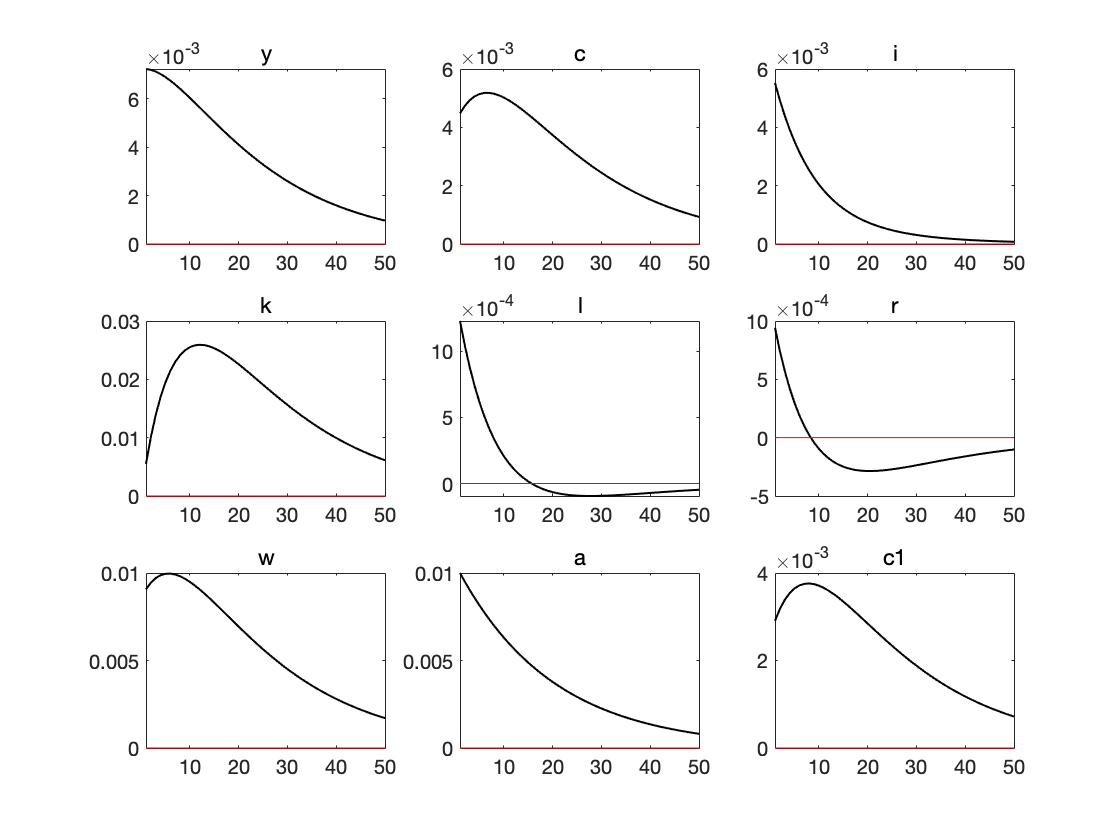
\includegraphics[width=\linewidth]{img/figure1.png}
    \caption{稳态结果模拟}
\end{figure}
\section*{第七题}
$\lambda$增大时,稳态水平下第一种类型的人消费增加,劳动时间明显下降;而对于响应函数,第一种类型的人消费的变化幅度降低,但整体和第二种类型的人消费的变化增大
\begin{table}[H]
    \centering
    \begin{tabular}{c|c|c|c}
        variable & $\lambda=0.1$ & $\lambda=0.5$ & $\lambda=0.9$ \\\hline
        y        & 0.559836      & 0.559836      & 0.715671      \\
        c        & 0.49519       & 0.49519       & 0.566914      \\
        c1       & 0.373893      & 0.373893      & 0.535901      \\
        c2       & 0.616488      & 0.616488      & 0.846025      \\
        i        & 0.129292      & 0.129292      & 0.165286      \\
        k        & 2.15487       & 2.15487       & 2.75477       \\
        l        & 0.393512      & 0.393512      & 0.366566      \\
        l1       & 0.393512      & 0.393512      & 0.366566      \\
        l2       & 4.29611e-08   & 4.29611e-08   & 6.44899e-08   \\
        r        & 1.03093       & 1.03093       & 1.03093       \\
        w        & 0.924732      & 0.924732      & 1.26904       \\
        a        & 1             & 1             & 1             \\
    \end{tabular}
\end{table}
\begin{figure}[H]
    \begin{minipage}{0.48\linewidth}
        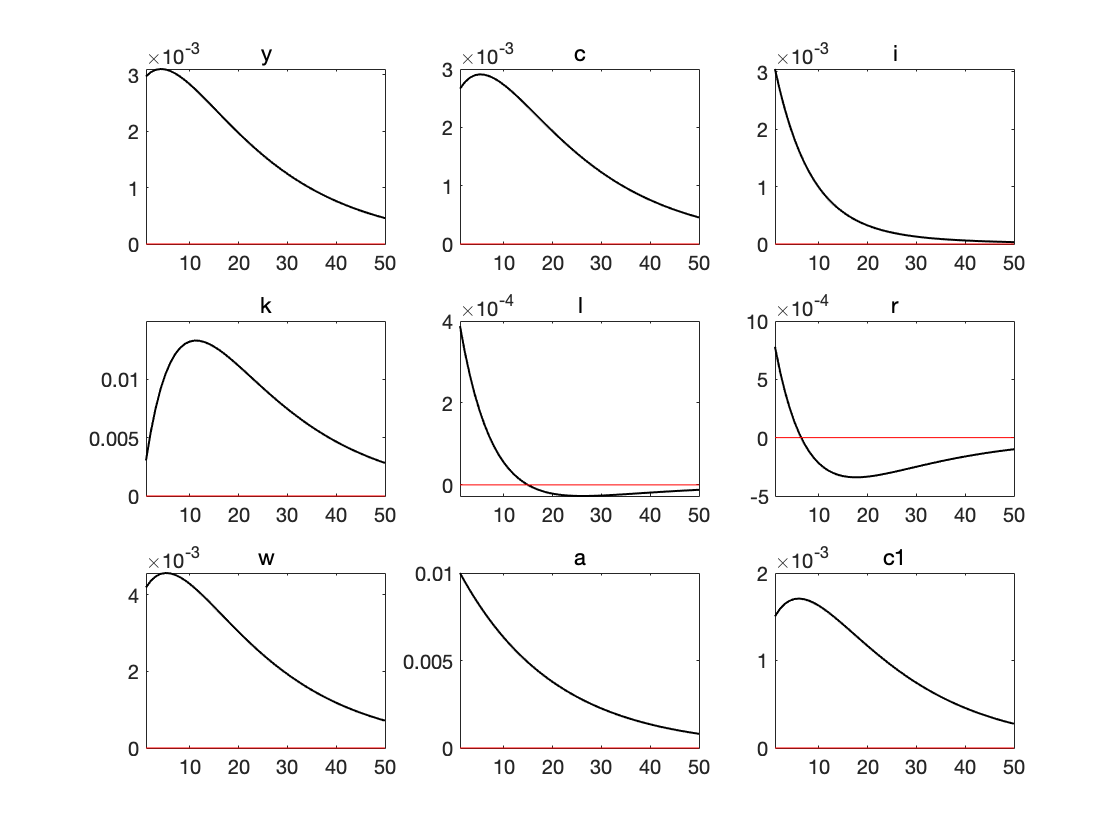
\includegraphics[width=\linewidth]{img/figure0.1.png}
        \caption{$\lambda=0.1$}
    \end{minipage}
    \begin{minipage}{0.48\linewidth}
        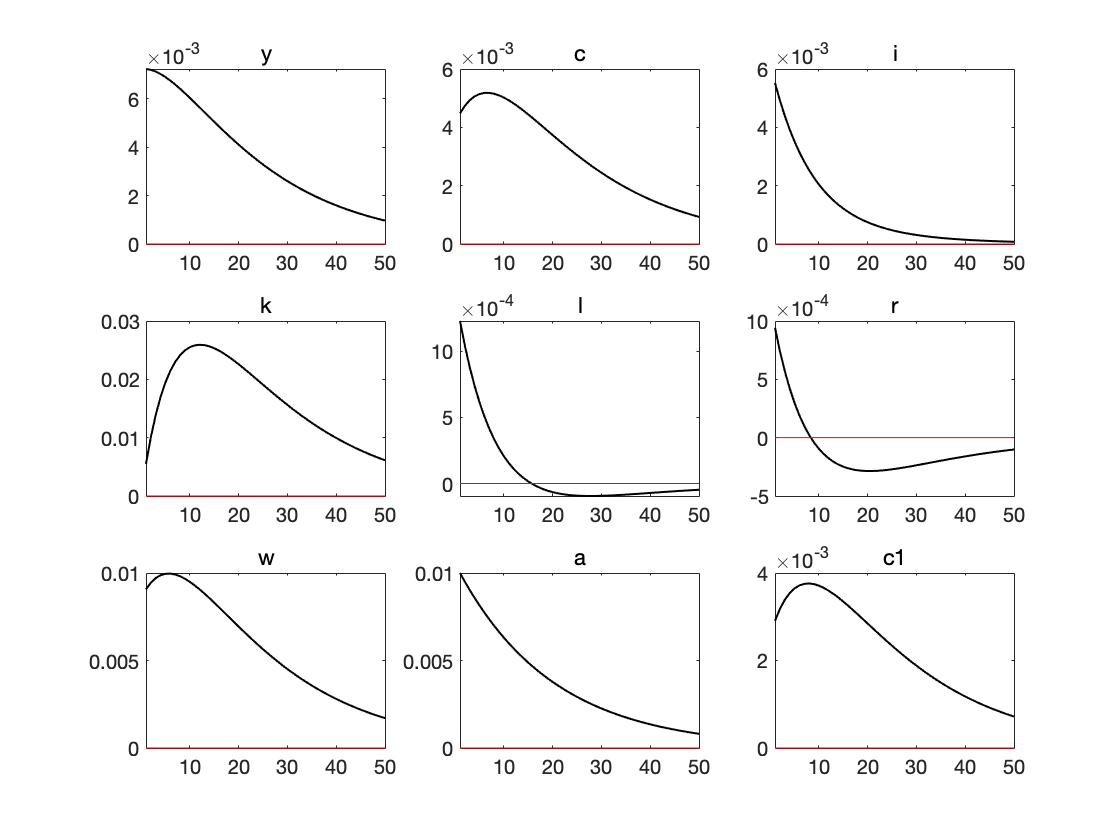
\includegraphics[width=\linewidth]{img/figure1.png}
        \caption{$\lambda=0.5$}
    \end{minipage}
    \begin{minipage}{0.48\linewidth}
        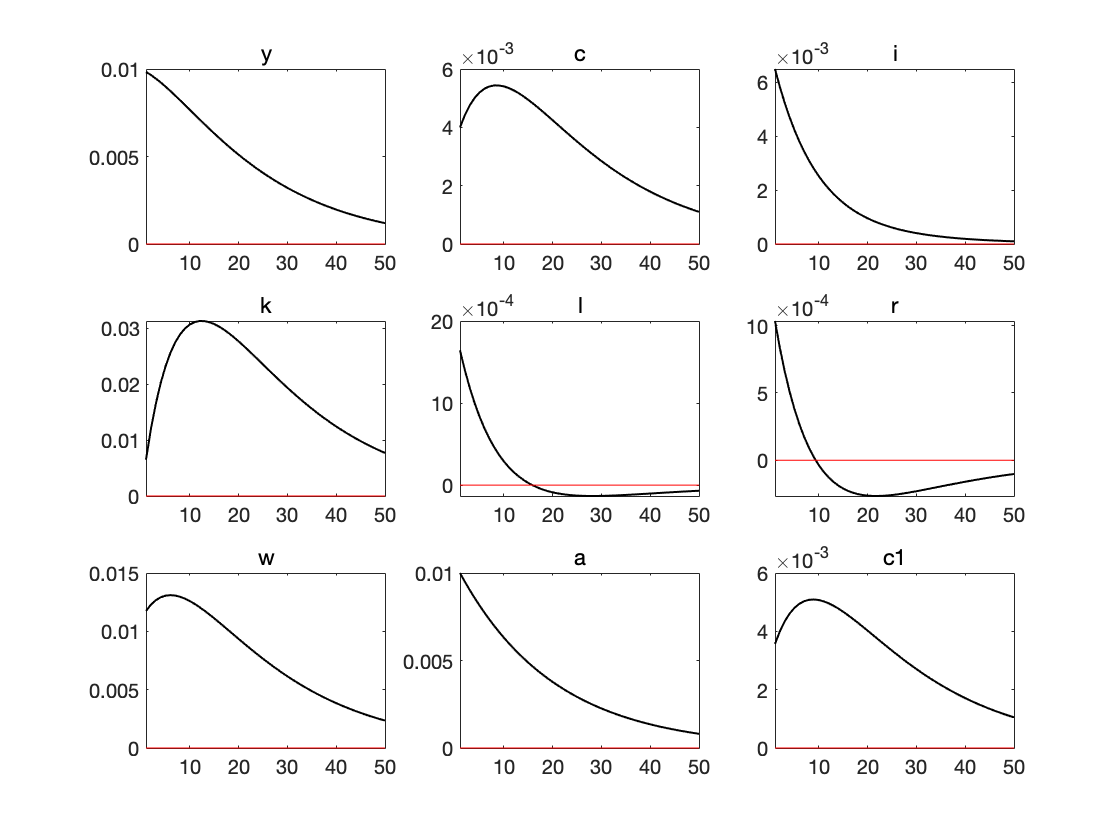
\includegraphics[width=\linewidth]{img/figure0.9.png}
        \caption{$\lambda=0.9$}
    \end{minipage}
\end{figure}
\end{document}
